\cleardoublepage

\chapter{Implementacion}
\label{makereference5}



\section{Instalación y configuración del nodo principal}
\label{makereference5.1}
 Utilizando los repositorios de distribuciones oficiales de Sistemas operativos de Raspberry Pi, descargamos la versión ``Lite'' de Raspbian. Para establecer una conexión SSH por terminal es necesario crear un fichero con nombre \verb|ssh| en la raiz de la unidad de almacenamiento donde previamente se haya montado la imagen descargada. La distribución de Raspbian originalmente estaba configurada por defecto con la conexión de SSH abierta en el puerto 22, pudiendo accederse con el usuario \verb|pi| y la contraseña \verb|raspberry|. Este dato era ignorado por los usuarios menos experimentados y esto supuso una brecha de seguridad en todos las distribuciones que no fueron configuradas a posteriori por los usuarios según las indicaciones de la propia \href{https://www.raspberrypi.org/documentation/configuration/security.md}{documentación de Raspberry}~\cite{securingyourraspberrypi}. En el primer arranque del SO de la Raspberry se establecerán las configuraciones básicas para las sucesivas conexiones SSH basadas en autenticación con claves privadas.

 fiware citas bitpex

 De las estrategias disponibles para esta configuración, se crearán las claves en el equipo remoto que se conectará a la Raspberry, entregando mediante la primera conexión SSH con terminal la clave pública y almacenando la clave privada en el equipo remoto, reduciendo así el riesgo de ser expuesta fuera del dominio local del equipo. Para disponer de flexibilidad de conexión independientemente del SO del equipo remoto, la clave privada tendra un formato OpenSSH, fácil de incluir en SO Windows ya sea mediante conversión de la clave a formato PPK o como fichero accesible para aplicaciones de desarrollo, transferencias de ficheros, y/o control de versiones que integran conexiones SSH configurables (GitHub, Filezilla, Eclipse, etc).

En Windows puede utilizarse aplicaciones de gestión de claves como 'puttygen'. En la sección de parámetros de generación de las claves se define SSH-2 RSA de 2048bits y en la sección de acciones pulsamos en 'genérate'. Tras unos movimientos aleatorios de ratón se generará la clave pública en el área de texto. Se deben guardar ambas claves mediante los botones 'save public key' y 'save private key'. Esta última será guardada con una contraseña definida en los inputs de la aplicación para tal fin. La clave privada será almacenada en formato PPK para ser rápidamente usada por aplicaciones de conexión por terminal remota como 'PUTTY'. Es recomendable exportar dicho fichero a formato OpenSSH mediante la misma aplicación de generación de claves, en la sección 'Conversions' del menú desplegable y seleccionando la opción 'Export OpenSSH key', definimos un nombre para el fichero de salida y pulsamos 'save'. Esta misma operación puede realizarse desde una terminal de un SO Linux mediante el comando \verb|ssh-keygen -t rsa| que generará por defecto la claves en el directorio \path{/home/username/.ssh/} bajo el nombre \verb|id_rsa.pub| e \verb|id_rsa| para las claves pública y privada respectivamente.

Al no disponer de interfaz mediante dispositivos I/O para una acceso local con la Raspberry, es necesario establecer una primera conexión de terminal remoto mediante SSH con usuario y contraseña. Este primer acceso nos permite establecer las reglas de conexión que se usarán en adelante en el fichero de configuración en la ruta \path{/etc/ssh/sshd_config} asi como la configuracion de cuentas de usuarios.

Las distribuciones de Raspbian disponen del usuario por defecto \verb|pi|. Esta cuenta de usuario esta incluido dentro del grupo de usuarios \verb|sudo|. En adelante se operará con una cuenta distinta que ha de generarse manualmente y adicionalmente eliminar la cuenta del usuario \verb|pi| para limitar brechas de seguridad. Como primer paso, crear el usuario \verb|sudo adduser kadaiser| e incluir al usuario en el grupo de usuarios \verb|sudo|. El fichero por defecto creado durante la instalación de la distribución situado en \path{/etc/sudoers} dispone de la directiva \verb|includedir /etc/sudoers.d| que debe ser descomentada en el fichero de configuración de \verb|sudo sudoers|, mediante el comando \verb|visudo|. Es necesario crear un fichero en la ruta \path{/etc/sudoers.d} con el siguiente formato de nombre \verb|010_kadaiser-nopasswd| cuyo contenido incluya la siguiente linea \verb|kadaiser ALL=(ALL) NOPASSWD: ALL| una vez se haya habilitado la directiva. Tras realizar las comprobaciones de que el nuevo usuario puede operar sin problemas con la nueva configuración de permisos, se elimina el fichero de permisos existente en \path{/etc/sudoers} para el usuario \verb|pi|, y su eliminación del sistema con el comando \verb|sudo deluser -remove-home pi|.

Para realizar la comunicación remota por terminal en SSH de manera más segura y cómoda, incluiremos un fichero con el contenido de la clave pública en una ruta manualmente definida dentro del 'home' del usuario kadaiser.

En concreto modificaremos el puerto de entrada para redirigir la conexión del puerto por defecto 22 a un valor más elevado (como por ejemplo el 45021). Esta decisión tiene como objetivo retrasar las técnicas de sondeo de puertos de un atacante hacia un servidor que admite conexiones externas. Un bot programado para encontrar servidores y marcarlos como objetivo de ataques escaneara puertos mediante evaluación de respuestas con paquetería ICMP. Igualmente un atacante puede determinar la naturaleza de los servicios ofrecidos por un servidor mediante herramientas como 'Nmap', al establecer valores elevados en los puertos, un rastreo incremental desde los valores más bajos llevará mas tiempo, permitiendo a las soluciones de seguridad (como un WFS) del servidor detectar el ataque con margen mayor de tiempo.

En este mismo fichero establecemos unos límites concretos en los valores de tiempo de gracia \verb|LoginGraceTime 5| de apenas 5 segundos, impedimos el acceso del usuario root desde una conexión externa \verb|PermitRootLogin no|, limitamos el número de intentos de conexión \verb|MaxAuthTries 3| y el número máximo de sesiones simultáneas \verb|MaxSessions|. Para admitir las conexiones SSH mediante una autentificación con clave es necesario habilitar la autentificación de clave pública \verb|PubkeyAuthentication yes| y definir la ruta del fichero con la clave publica almacenada localmente en el servidor \verb|AuthorizedKeysFile| \path{.net/.aut} (véase que en este caso hemos definido una ruta manualmente indicando que la clave pública se encuentra en un fichero oculto nombrado \verb|aut| en la ruta \path{/home/pi/.net}). Como refuerzo adicional configuramos el servidor para denegar todo intento de conexión mediante contraseña plana \verb|PasswordAuthentication no|, y adicionalmente limitar el acceso sólo a las cuentas de usuarios designadas \verb|AllowUsers kadaiser|. Definidos los nuevos cambios de configuración, es necesario reiniciar el servicio.

Establecemos la capacidad de la Raspberry Pi 3 para su módulo de comunicación wifi de actuar como punto de acceso en modo NAT~\cite{raspberrypiasaccesspoint}. Se configura una red con acceso vía usuario y contraseña, con WPA2 y gestión de claves WPA-PSK. De esta forma, el nodo será capaz de desplegar una red inalámbrica que permitirá a otros dispositivos incorporarse a la suite domótica.

Descargamos la paquetería de Adafruit para el primer sensor de pruebas, el sensor DTH11 de temperatura y humedad.
Se requiere un montaje sencillo.
\begin{figure}[hbt!]
\centering
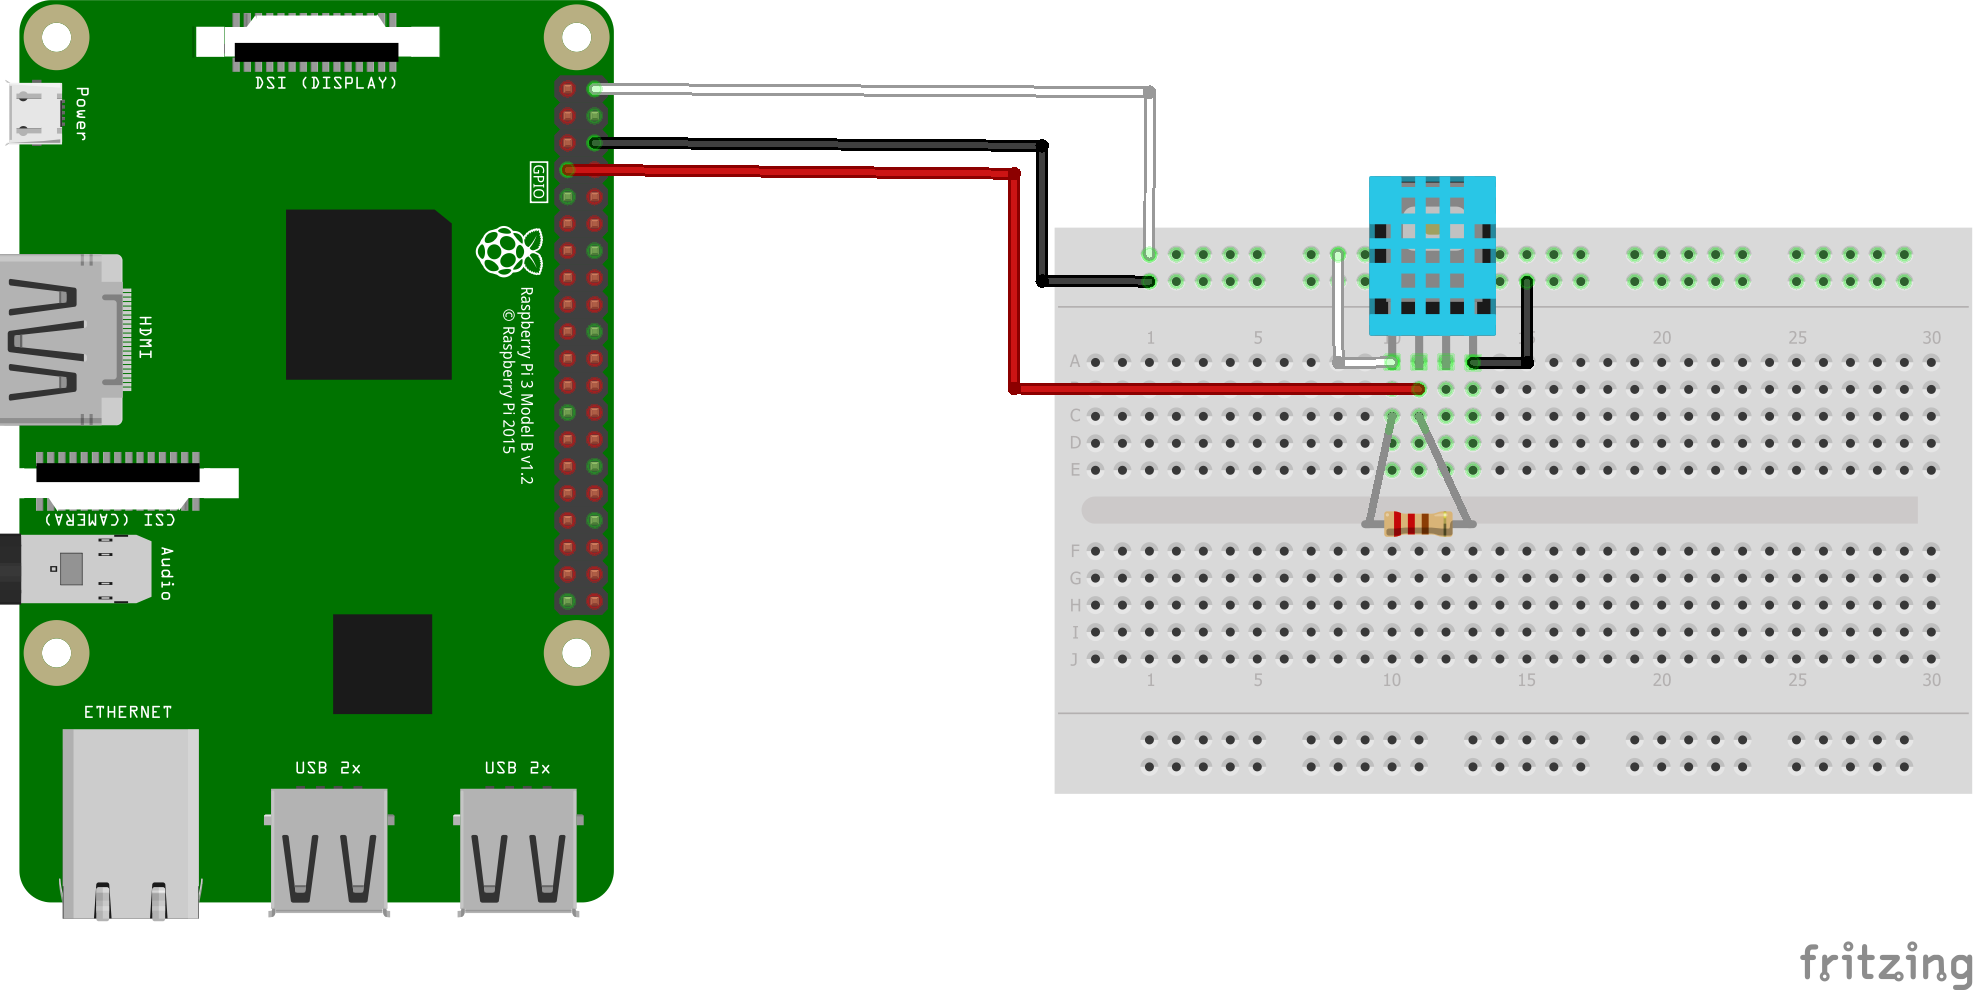
\includegraphics[height=2.5in]{figures/nodo_1.png}
\end{figure}

Clonamos la librería del sensor, nos ubicamos en la ruta descargada \verb|cd Adafruit_Python_DHT| e instalamos la librería \verb|sudo python setup.py install|, previamente instalamos las dependencias de la librería para su instalación \verb|sudo apt-get install python-setuptools| considerando que tenemos la versión de python 2.7.3, esto permitirá instalar la librería de python para el sensor DHT version 1.4. Se debe realizar una prueba de contacto con un script que nos muestre la información por pantalla para verificar que las conexiones del sensor a la rapsberry son correctos. Este primer script es un bucle infinito de mediciones de temperatura y humedad cada poco segundos. Hay una justificación para elegir un bucle sobre una única medida del sensor y está fundamentada en el margen de error inicial de las medidas. Si bien el sensor DTH11 es una opción muy común por su bajo coste y facilidad de implementación (este sensor se caracteriza por tener la señal digital calibrada por lo que asegura una alta calidad y una fiabilidad a lo largo del tiempo, ya que contiene un microcontrolador de 8 bits integrado. Está constituido por dos sensores resistivos (NTC y humedad) - revisar esta info y contrastarla contra ésta: \url{ https://programarfacil.com/blog/arduino-blog/sensor-dht11-temperatura-humedad-arduino/}), ademas de manejar señales digitales que no se ven afectadas por las fluctuaciones de voltaje, tiene algunas contrapartidas que deben tenerse en cuenta. Se necesita un tiempo mínimo de espera entre medidas (de al menos 1 segundo), hecho que no agrava particularmente su desempeño en entornos cerrados como una casa, ya que las variaciones de temperatura y humedad no son bruscas, aun así existen estrategias para reducir estos tiempos, por ejemplo, usar la función millis() de Arduino, el cual nos da el tiempo en milisegundos desde que empieza a ejecutarse el código, De esta forma evitamos la pausa de los 2 segundos, pero no el tiempo que demora en hacer la lectura, que es de aproximadamente  250 milisegundos, el cual lo pueden notar si realizan el ejemplo anterior, en donde se hace parpadear el led interno de la placa (Pin 13) con pausas de 100ms (tomado de \url{https://naylampmechatronics.com/blog/40_Tutorial-sensor-de-temperatura-y-humedad-DHT1.html}). Otro problema que abordar es que las primeras lecturas tienen un margen de error de unos +-2 grados Celsius y +-5\% de humedad relativa en las primeras 4 lecturas. Esto generará un problema a la hora de tomar lecturas instantáneas si el sensor no se encuentra ya operando cuando se solicita el dato. Como estrategia, haremos que el sensor tome medidas indefinidamente y los vuelque en un fichero/BBDD para recortar los tiempo de respuesta, evitando así esperar a que el sensor haga la toma de medidas en el momento+ de solicitud y sacándolas en su lugar del último registro que tengamos. Un último problema con el que hay que lidiar es su baja precisión limitada a enteros, por lo que no podemos esperar obtener un dato preciso a la décima de la temperatura y humedad. Esto sin embargo no es un problema real dada la naturaleza del proyecto, ya que no necesitamos un grado de precisión menor a la unidad para tomar acciones o informar al usuario.

En orden de subir sketcs a una arduino desde una Raspeberry Pi, es necesario isntalar las paqueterias del compilardor \verb|sudo apt-get install arduino-mk|, tras la instalación, en la ruta \verb|/usr/sahre/arduino| pueden encontrar binarios y una capeta llamada \verb|examples| que permiten cargan sketchs inmediatamente para comprobar el correcto funcionamiento del la placa microcontroladora. Para compilar dicho sketcs se necesita referenciar el fichero arduino.mk. De los ejemplo podemos verificar rampidamente el correcto funcionamiento de la microcontroladores utilizamos el mas basico de los sketcs, situado en \verb|/usr/share/arduino/examples/01.Basic/Blink/Blink.ino|, este ejemplo es muy basico, un loop que enciende y apaga el led integrado en la placa microcontroladora cada 1000 milisegundos. Este , es por defecto el sketch que generelamente los disitntos fabricantes de placas microcontroladoras de con procesador ATmega328P suelen dejar cargado a modo de test. Alterando el valor basico de sleep entre lineas de encendido y apagado a un valor menor como 50 milisegundos se puede comprobar si la comunicación del puerto com, y el compilador suben correctamente el codigo a la placa. Es importante verificar este punto antes de continuar y esta simple prueba cofirma que la configuración actual esta bien.

Para facilitar el proceso de subida de codigo a la placa de arduino, crearemos un Makefile hijo que enlace parametros al compilador.


Ahoera bien, tengamos en cuenta que las especificaciones del modulo esp8266 de wifi conectado a arduino requieren de una laimentación de 3.3V que pueden ser suministrados por la placa microcontroladora, sin embargo, esto nos deja con un problema de intensidad en la alimentación del modulo, ya que el pin de 3.3V disponible en la placa posees un amperaje de 50mA y se requieren de unos 200mA para garatizar una comunicación estable.

--Datos importantes para ahcere que funcionen ch340

sudo apt-get install git raspberrypi-kernel-headers build-essential dkms
https://github.com/juliagoda/CH341SER
nano328
